\newcommand{\Titelpdf}{LBS_Bericht_Kaur_Zeyse}
\newcommand{\DeinName}{Sumit Kaur und Simeon Zeyse}
\newcommand{\Matrikelnummer}{6059167 und 6056745}
\newcommand{\TitelArbeit}{Optimieren einer Trajektorie mit absoluten 5G Koordinaten\\[0.4mm]}
\newcommand{\PrueferEins}{M.Sc. Hossein Shoushtari}
\newcommand{\artDerArbeit}{Location Based Service}
\newcommand{\Datum}{\today}

%%%%%%%%%%%%%%%%%%%%%%%%%%%%%%%%%%%%%%%%%%%%%%%%%%%%%%%
%																					%
%	In dieser Datei werden alle Packages eingebunden, 	%
% welche f�r das Dokument n�tig sind. Desweiteren 		%
% werden die Dokumentinformationen gesetzt.						%
%																											%
%%%%%%%%%%%%%%%%%%%%%%%%%%%%%%%%%%%%%%%%%%%%%%%%%%%%%%%
%

%
\documentclass[pdftex, 		a4paper, 		% DIN A4 verwenden
							titlepage,	    % separate Titelseite
							%draft,			% Draft-Version, keine Bilder im pdf!
							emulatestandardclasses,
							final,			% Final-Version
							oneside,		% zweiseitiger Druck %X
							11pt,			% Schriftgr��e 12pt
							%BCOR20mm,		    			    %X
							DIV=calc,		
							headsepline,	
							%tocbasic,
							%openany,
							%pointlessnumbers
							]{article}	%	KOMAScript scrbook-Dokumentklasse							
%%%%%%%%%%%%%%%%%%%%%%%%%%%%%%%%%%%%%%%%%%%%%%%%%%%%%%%%
%	Einbinden der Pakete 
%%%%%%%%%%%%%%%%%%%%%%%%%%%%%%%%%%%%%%%%%%%%%%%%%%%%%%%%
\usepackage[a4paper, left=2.5cm, right=2.5cm, top=3cm, bottom=3cm, bindingoffset=0mm]{geometry}
%bindingoffset=15mm]

\usepackage[ngerman,english]{babel}
\usepackage{multirow}
\usepackage{amsmath}
\usepackage{amssymb}
\usepackage[pdftex]{graphicx}
\usepackage{chngcntr}
\counterwithin{table}{section}
\counterwithin{figure}{section} %X
\counterwithin{equation}{section} %X
\usepackage{booktabs}
% PDF Dateien einbinden
\usepackage{pdfpages}
\usepackage{textcomp} 
\usepackage{upgreek}%kein Kursiv mehr
\pdfminorversion=6
\pdfcompresslevel=9

% Abstand zu Section...
%\RedeclareSectionCommand[beforeskip=-1.5\baselineskip,afterskip=.5\baselineskip]{section}
%\RedeclareSectionCommand[beforeskip=-.75\baselineskip,afterskip=.5\baselineskip]{subsection}
%\RedeclareSectionCommand[beforeskip=-.5\baselineskip,afterskip=.25\baselineskip]{subsubsection}
%\RedeclareSectionCommand[beforeskip=.5\baselineskip,afterskip=-1em]{paragraph}

\usepackage{textcomp} %griechische Alphabet nicht kursiv

%Einige Pakete haben Probleme mit dem Komaskript.
\usepackage{scrhack} 

\usepackage{xcolor}
\definecolor{urlLinkColor}{rgb}{0,0,0.5}
\definecolor{LinkColor}{rgb}{0,0,0}

\usepackage{abstract} %Abstrakt

\usepackage{csquotes}
\usepackage[backend=biber,style= apa, sortcites = true]{biblatex}

\newcommand\ifintextcite{\ifdefstring{\blx@delimcontext}{textcite}} %parencite und textcite unterschiedlich
\DefineBibliographyStrings{german}{
	andothers = {\ifintextcite{and others}{et\addabbrvspace al.}},
%	nodate = {o.D.},
%	backrefpage  = {\lowercase :}
%	pages = {:}
}
\setlength{\bibitemsep}{12pt}
\addbibresource{source/bib/references.bib}
	
\usepackage[latin1]{inputenc} % Umlaute %  
\usepackage[scaled]{berasans}				% Schriftfamilie
\renewcommand{\rmdefault}{phv}
\renewcommand{\sfdefault}{phv}

% Grafikpaket
\usepackage{makeidx}   				% Paket zur Erzeugung eines Index
\usepackage[normalem]{ulem}   % bietet Unterstreichungsvarianten
%\usepackage{picins} 					% Bilder im Absatz platzieren
\usepackage[T1]{fontenc}			% Erweiterten Zeichensatz aktivieren
\usepackage{multido}					% erm�glicht Schleifenartiges wiederholen von Befehlen
\usepackage{mdwlist}					% erm�glicht das Setzen des Z�hlers bei Aufz�hlungspunkten
\usepackage{paralist}					% Paket f�r Aufz�hlungen, erweitert Enumerate-Paket
\usepackage{longtable}				% mehrseitige Tabellen
%\usepackage{tocloft}
\parindent0pt           			% verzichte auf Einr�cken der ersten Zeile
\parskip2ex            	% Abstand zwischen den Abs�tzen

\usepackage{floatflt,epsfig} %text neben Bild

%\usepackage{setspace}					% Paket zum Einstellen des Zeilenabstands
%\doublespacing								% doppelter Zeilenabstand
\linespread{1.5}


\usepackage{color}
\definecolor{hcu-blau}{RGB}{54, 141, 207}

% Farbeinstellungen f�r die Links im PDF Dokument.
%
\makeindex

%-----------Paket f�r absolute Positionierung von Grafiken------------------
\usepackage[absolute]{textpos}
\setlength{\TPHorizModule}{1mm}
\setlength{\TPVertModule}{\TPHorizModule}

%-----------Aufz�hlungen und Einstellungen f�r Sourcecode-------------------
%\usepackage[savemem]{listings} %Bei wenig Arbeitsspeicher dies Option [savemem] aktivieren.
\usepackage{listings}
\lstloadlanguages{TeX,XML, Java} % TeX sprache laden, notwendig wegen option 'savemem'
\lstset{%
	language=[LaTeX]TeX,     % Sprache des Quellcodes ist TeX
	numbers=left,            % Zelennummern links
	stepnumber=1,            % Jede Zeile nummerieren.
	numbersep=5pt,           % 5pt Abstand zum Quellcode
	numberstyle=\tiny,       % Zeichengr�sse 'tiny' f�r die Nummern.
	breaklines=true,         % Zeilen umbrechen wenn notwendig.
	breakautoindent=true,    % Nach dem Zeilenumbruch Zeile einr�cken.
	postbreak=\space,        % Bei Leerzeichen umbrechen.
	tabsize=2,               % Tabulatorgr�sse 2
	basicstyle=\ttfamily\footnotesize, % Nichtproportionale Schrift, klein f�r den Quellcode
	showspaces=false,        % Leerzeichen nicht anzeigen.
	showstringspaces=false,  % Leerzeichen auch in Strings ('') nicht anzeigen.
	extendedchars=true,      % Alle Zeichen vom Latin1 Zeichensatz anzeigen.
	backgroundcolor=\color{ListingBackground}} % Hintergrundfarbe des Quellcodes setzen.


\lstset{
  basicstyle=\small\ttfamily,
  columns=fullflexible,
  showstringspaces=false,
  %commentstyle=\color{gray}\upshape
}
%neue Lang definieren, als Bsp.
\lstdefinelanguage{XML-changed}
{
  basicstyle=\footnotesize\ttfamily\bfseries,
  morestring=[b]",
  morestring=[s]{>}{<},
  morecomment=[s]{<?}{?>},
  stringstyle=\color{black},
  identifierstyle=\color{darkblue},
  keywordstyle=\color{cyan},
  morekeywords={xmlns,version,type}% list your attributes here
}

%-----------Caption Package-------------------
\usepackage{caption}
\usepackage{subcaption}
\DeclareCaptionFont{hcu-blau}{\color{hcu-blau}}

\usepackage{silence}
\WarningFilter{scrbook}{Usage of package `fancyhdr'}

\usepackage[labelfont = {bf,it}, font={footnotesize,it}, labelsep = space]{caption} %Beschirftung Tabelle/Abbildung

%\usepackage[labelfont={hcu-blau,{bf}}]{caption}
\renewcommand{\arraystretch}{1.0}   %tabellenabstand

\usepackage[labelfont = {bf,it}, font={footnotesize,it}, labelsep = space]{subcaption}

%-----------Header+Footer---------------------------------------------------
%\usepackage{fancyhdr}					
%\pagestyle{fancy}
%\fancyhf{}							
%\lhead{\leftmark}
%\rhead{\DeinName}
%\rfoot{\thepage} 
%\fancyfoot[EL]{\thepage}   %Seitenzahl abwechselt
%\fancyfoot[OR]{\thepage}   %Seitenzahl abwechselt
%\renewcommand{\headrulewidth}{0.2pt} % Kopflinie
%\renewcommand{\sectionmark}[1]{\markleft{\arabic{chapter}.\arabic{section}\ #1}}

%--------------------------------------------------------------------------------

\usepackage{scrlayer-scrpage}
\pagestyle{scrheadings}
\clearpairofpagestyles

\ohead{\pagemark}
%\chead{Kopfzeile Mitte}
\ihead{\leftmark}
%\ifoot{Fu�zeile innen}
%\cfoot{Fu�zeile Mitte}
%\ofoot{\pagemark}

%\renewcommand*\chapterpagestyle{scrheadings}
\renewcommand{\sectionmark}[1]{\markleft{\arabic{section}\ #1}}
%--------------------------------------------------------------------------------

% -------F�r ToDo-Notes--------------------------------------------------------------------
\usepackage[color=red, shadow]{todonotes} % ", disable" deaktiviert ToDo-Notes
%Vereinfachtes "Inline-Todo"
\newcommand{\td}[1]{{\todo[inline]{#1}}}
\newcommand{\tdu}[1]{{\todo[inline, color=green!40]{#1}}}

%--------F�r Links-------------------------------------------------------------------------
%--------HyperRef konfigurieren-------------------------------------------------------------------------

\usepackage[
	pdftitle={\Titelpdf},
	pdfauthor={\DeinName},
	pdfsubject={\TitelArbeit},
	pdfcreator={MiKTeX, LaTeX with hyperref and KOMA-Script auf Basis der Vorlage von seiler.it},
	pdfkeywords={Bachelorarbeit, Hamburg, HafenCity Universit�t},%weitere Keywords hier einf�gen
	pdfpagemode=UseOutlines,%                                  
	pdfdisplaydoctitle=true,%                                  
	pdflang=de%                                              
]{hyperref}

\hypersetup{%
	colorlinks=true,%        Aktivieren von farbigen Links im Dokument (keine Rahmen)
	linkcolor=LinkColor,%    Farbe festlegen.
	citecolor=LinkColor,%    Farbe festlegen.
	filecolor=LinkColor,%    Farbe festlegen.
	menucolor=LinkColor,%    Farbe festlegen.
	urlcolor=LinkColor,%     Farbe von URL's im Dokument.
	bookmarksnumbered=true%  �berschriftsnummerierung im PDF Inhalt anzeigen.
}


% Beginn des Dokuments
\begin{document}
\clearpage
\nocite{*}
\pagenumbering{roman} 
\tableofcontents
\clearpage
\listoffigures
\clearpage
\pagenumbering{arabic}
\setlength\abovedisplayskip{8pt}
\setlength\belowdisplayskip{8pt}
\section{Einleitung}
Vorallem in un�bersichtlichen und unbekannten Geb�uden kann die Verwendung von Indoor Navigation n�tzlich sein, um die Positionen von Menschen oder Objekten zu verfolgen. Das Problem bei der Navigation im Geb�ude ist der schlechte bis fehlende GNSS-Empfang. Weshalb das sonst �bliche Verfahren, mittels Satellitennavigation im Geb�ude meistens keine zufriedenstellende Positionsl�sung bietet und somit meistens keine zuverl�ssige M�glichkeit bei der Indoor Navigation darstellt. Da Inertiales Navigationssysteme (INS) ohne GNSS-Signale auskommen, k�nnen sie hervorragend in der Indoor-Navigation eingesetzt werden. Daf�r wird ein einfacher Bewegungssensor ben�tigt, welcher sich beispielsweise in einem Ortungssystem f�r gehende Personen befindet, das so genannte \textit{Personal Dead Reckoning (PDR)}-System. Das PDR-System verwendet eine Inertialmesseinheit (IMU). Diese wird am Schuh des Nutzers befestigt und liefert Informationen wie die Schrittl�nge und Schrittrichtung. Diese Informationen k�nnen dabei helfen den Standpunkt des Nutzers relativ zu einem bekannten Referenzpunkten in Echtzeit zu ermitteln \parencite{borenstein2007}. In dieser Arbeit werden sogenannte 5G-Koordinaten als bekannte Referenzpunkte verwendet.

Nachteile eines PDR-System ist das sie durch akkumulierte Messfehlern einen Drift aufweisen (siehe Abbildung \ref{fig:pdr}). Wie man sieht, kann die PDR Trajektorie der Ground Truth am Anfang f�r etwa 10 - 15 Meter relativ genau folgen. Anschlie�end driftet die PDR Trajektorie allerdings zunehmend nach rechts ab.
\begin{figure}[h!]
	\centering
	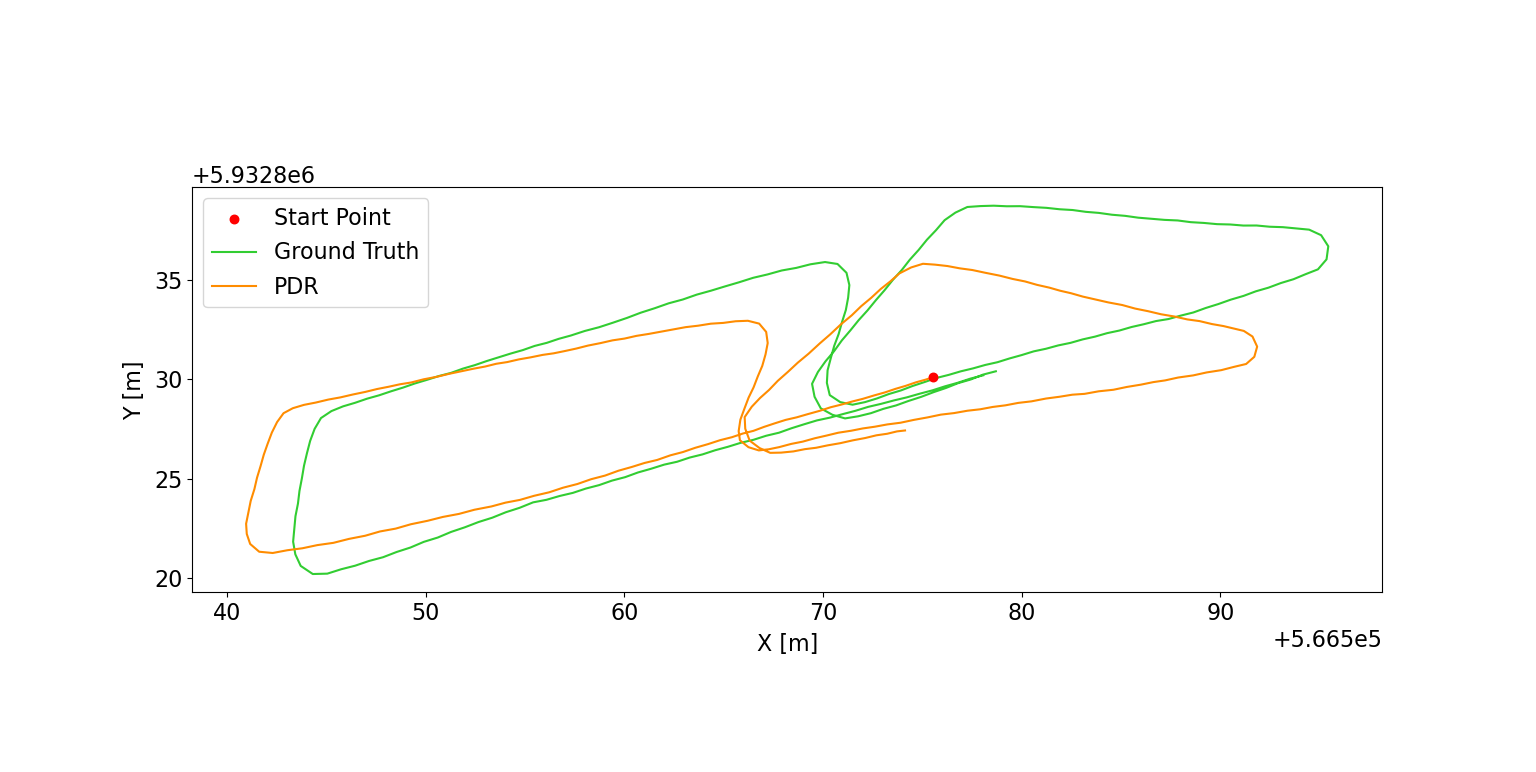
\includegraphics[width=0.8\linewidth]{source/images/pdr_drift}
	\caption{PDR Trajektorie und Ground Truth}
	\label{fig:pdr}
\end{figure}
Dies liegt daran, dass sie der Fehler der Schrittrichtung immer akkumuliert und so auch bei einem geringen Fehler mit der Zeit ein erheblicher Drift entsteht. Insgesamt l�sst sich aber feststellen, dass die PDR Trajektorie f�r kurze Distanzen sehr gut geeignet ist. Dieser Drift kann jedoch mit Hilfe regelm��iger Abgleichung von Referenzpunkten (in diesem Fall absolute 5G-Koordinaten) korrigiert werden. 

Durch diese Abgleichung entsteht eine optimierte Trajektorie, welche dann sowohl aus 5G-Koordniaten und PDR-Messwerten besteht. So nutzt man die 5G-Koordinaten zur absoluten Positionsbestimmung, w�hrend die PDR-Messungen durch ihre h�here Messrate daf�r sorgen, dass der Verlauf der Trajektorie der Ground Truth n�hert kommt. Daf�r sind in der Geod�sie Optimierungsans�tze wie das Kalman-Filter oder die Methode der kleinsten Quadrate (engl.: Least-Square) h�ufig im Einsatz.

Diese Arbeit besch�ftigt sich daher mit der Frage wie sich die Ergebnisse einer Ausgleichung von Personal Dead Reckoning (PDR) mittels dem dynamischen Kalman-Filter und der Least-Square Methode unterscheiden?

Auch andere Arbeiten besch�ftigen sich mit solchen Thema. Das Paper \textcite{kjellson2021} z.B. beschreibt Deep-Learning-Methoden sowohl f�r die Sch�tzung von absoluten Positionen als auch f�r die Durchf�hrung einer Koppelnavigation f�r Fu�g�nger (PDR). Beiden Ans�tze wurden zur Optimierung der Trajektorie mit Hilfe der gewichteten kleinsten Quadrate (engl.: weighted least square) kombiniert.

Einige Herausforderungen, die w�hrend der Bearbeitung des Themas entstanden sind, war weniger das theoretische Verst�ndnis, sondern viel mehr die Implementation in Python. Oft kommt es beim Programmieren zu Fehlermeldungen, die nicht immer so schnell zu l�sen sind. 

In diese Arbeit ist aufgeteilt in drei Oberkapitel: Methodologie, Implementation und Fazit und Ausblick. In dem Kapitel Methodologie werden die generellen Konzepte des Diskreten Kalman-Filters, des extended Kalman-Filter und der des Weighted Least-Square Methode dargestellt. Bei der Implementation wird die detailiierte Ausf�hrung der Arbeitsschritte samt ihrer Ergebnissen vorgestellt. Damit werden die Ergebnisse der unterschiedlichen Verfahren miteinander verglichen. Zum Schluss werden die Ergebnisse zusammengefasst und kritisch analysiert. Als Ausblick wird/werden zuk�nftige Forschungsperspektiven dargelegt. 

\textcolor{red}{Was sind die Anwendungsbereiche des Themas?\\Was sind die bisherigen Herausforderungen?}

\section{Methodologie}
In diesem Kapitel werden die theoretischen Methoden und allgemeinen Konzepten des Kalman Filters und der Least Square-Methode beschrieben. 

\subsection{Das Kalman Filter}
W�hrend die meisten Systeme mit zahlreichen Sensoren ausgestattet sind f�hren diese mit Hilfe von Messungen eine Sch�tzung der unbekannten Parameter aus. Dabei kann es herausfordernd sein eine genaue und pr�zise Sch�tzung dieser Unbekannten unter Ber�cksichtigungen ihrer Unsicherheiten durchzuf�hren. Daf�r wird nicht selten der Kalman-Filter zur Hilfe genommen. Er findet dort Anwendung, wo bestimmte Sensoren nicht funktionieren oder sogar ausfallen und man dennoch die Systemgr��en sch�tzen m�chte. Das Kalman-Filter liefert somit eine Vorhersage des zuk�nftigen Systemzustands auf der Grundlage vergangener Sch�tzungen.

Der Filter ist nach Rudolf E. K�lm�n (19. Mai 1930 - 2. Juli 2016) benannt wurden. Im Jahr 1960 ver�ffentlichte K�lm�n seine ber�hmte Arbeit, in der er eine rekursive L�sung f�r das lineare Filterproblem mit diskreten Daten beschrieb \parencite{kalman}.

Bei dem Kalman Filter unterscheidet man zwei Arten von Filter: der statische und der dynamische Kalman Filter. Diese Arbeit wird sich mit dem dynamischen Kalman Filter auseinander setzen. Dieser setzt sich aus einem Beobachtungsmodell und einem Bewegungsmodell zusammen. Bei dem Beobachtungsmodell handelt es sich um Beobachtungen und ihre Unsicherheiten. Bei dem Bewegungsmodell wird auch von einer Pr�diktion (dynamisches Modell) und ihren Unsicherheiten gesprochen. Aus ihr erfolgt dann die Sch�tzung des Zustandes. Wenn sowohl Beobachtungsmodell als auch Bewegungsmodell linear sind wird der diskrete Kalman Filter verwendet. Wenn beide Modelle nicht-linear sind findet der Extended Kalman Filter Anwendung. 

\subsubsection{Diskreter Kalman-Filter (lineares Modell)}\label{subsub_diskret}
Bei dem diskreten Kalman-Filter ist die Idee die Beobachtungen zu bestimmten (diskreten) Zeitpunkten mit einem Bewegungsmodell zu kombinieren. Das Bewegungsmodell pr�diziert dann den Zustandsvektor ausgehend von der Sch�tzung des vorherigen Schrittes. Generell werden vier Schritte ben�tigt: die Pr�diktion, die Innovation, die Kalman-Gain-Matrix und das Update \parencite{teil1}. 

Das generelle Beobachtungsmodell sieht wie folgt aus:
\begin{equation}
\boldsymbol{l}_{i+1} = \boldsymbol{A}_{i+1}\boldsymbol{x}_{i+1} + \boldsymbol{e}_{i+1} \text{,}
\end{equation}
mit $\boldsymbol{l}$ = Beobachtungen/Messungen, $\boldsymbol{A}$ = Designmatrix, $\boldsymbol{x}$ = unbekannte Parameter und $\boldsymbol{e}$ = Residuen (Beobachtungsrauschen). Die Designmatrix beinhaltet die partiellen Ableitungen der Beobachtungsgleichungen nach den Parametern. Bei den Residuen handelt es sich um die negierten Verbesserungen. Sie sind normalverteilt mit einem Erwartungswert von 0. 

Das hier verwendete Bewegungsmodell sieht wie folgt aus:
\begin{equation}\label{x_i+1_allg}
\boldsymbol{x}_{i+1} = \boldsymbol{T}_i\boldsymbol{x}_i + \boldsymbol{C}_i\boldsymbol{w}_i \text{,}
\end{equation}
mit $\boldsymbol{T}$ = Transitionsmatrix (pr�diziert Bewegung von einem Zeitpunkt zum n�chsten), $\boldsymbol{w}$ = St�rgr��e (Unsicherheit im Bewegungsmodell: Rauschen), $\boldsymbol{C}$ = St�rgr��enmatrix (Auswirkung dieser Unsicherheit auf die Pr�diktion des Zustandes). Da wir annehmen, dass die Unsicherheiten im Bewegungsmodell ausreichend von den Varianzen der gesch�tzten Parameter abgedeckt werden, wird die Formel \ref{x_i+1_allg} durch die folgende Formeln ersetzt:
\begin{equation}\label{x_i+1}
\boldsymbol{x}_{i+1} = \boldsymbol{T}_i\boldsymbol{x}_i.
\end{equation}

In der Pr�diktion wird der aktuelle Schritt mit den Daten des vorherigen Schrittes und der Transitionsmatrix berechnet. Die Transitionsmatrix beinhaltet die partiellen Ableitungen der pr�dizierten Gr��en nach den Sch�tzungen des vorigen Schrittes. Die zugeh�rige Kovarianzmatrix wird mit Hilfe des Varianzfortpflanzungsgesetzes (VFG) berechnet. Dabei wird sich die Frage gestellt welche Trajektorie des Fahrzeugs das Bewegungsmodell voraus sagt. 
\begin{equation}
\boldsymbol{\bar{x}}_{i+1} = \boldsymbol{T}_i +\boldsymbol{\hat{x}}_{i}\\
\end{equation}
\begin{equation}
\boldsymbol{\Sigma}(\boldsymbol{\bar{x}}_{i+1}) = \boldsymbol{T}_i\boldsymbol{\Sigma}(\boldsymbol{\hat{x}}_{i})\boldsymbol{T}_i^T + \boldsymbol{C}_i\boldsymbol{\Sigma}(\boldsymbol{w}_{i})\boldsymbol{C}_i^T\\
\end{equation}
In dem 2. Schritt der Innovation wird geschaut wie sehr die eigentlichen Beobachtungen von der zuvor berechneten Pr�diktion abweichen, daf�r wird die Differenz der Pr�diktion zu den Beobachtungen berechnet und auch hier wird mit Hilfe des VFGs die Kovarianzmatrix gerechnet. 
\begin{equation}
\boldsymbol{d}_{i+1} = \boldsymbol{l}_{i+1} - \boldsymbol{A}_{i+1}\boldsymbol{\bar{x}}_{i+1}
\end{equation}
\begin{equation}
\boldsymbol{\Sigma}(\boldsymbol{d}_{i+1}) = \boldsymbol{\Sigma}(\boldsymbol{l}_{i+1}) + \boldsymbol{A}_{i+1}\boldsymbol{\Sigma}(\boldsymbol{\bar{x}}_{i+1})\boldsymbol{A}_{i+1}^T
\end{equation}
Dann folgt die Berechnung der Kalman Gain Matrix, welche die relative Gewichtung von Pr�diktion und Beobachtungen anhand der jeweiligen Genauigkeiten beinhaltetet. Die zugeh�rige Kovarianzmatrix des Updates wird auch wieder mit Hilfe des VFGs berechnet.
\begin{equation}
\boldsymbol{K}_{i+1} = \boldsymbol{\Sigma}(\boldsymbol{\bar{x}}_{i+1})\boldsymbol{A}_{i+1}^T\boldsymbol{\Sigma}^{-1}(\boldsymbol{d}_{i+1})
\end{equation}
In dem vierten und letzten Schritt dem Update wird ein gewichtiets Mittel aus der Pr�diktion und der Innovation errechnet.
\begin{equation}
\boldsymbol{\hat{x}}_{i+1} = \boldsymbol{\bar{x}}_{i+1} + \boldsymbol{K}_{i+1}\boldsymbol{d}_{i+1}
\end{equation}
\begin{equation}
\boldsymbol{\Sigma}(\boldsymbol{\hat{x}}_{i+1}) = [\boldsymbol{I}-\boldsymbol{K}_{i+1}\boldsymbol{A}_{i+1}]\boldsymbol{\Sigma}(\boldsymbol{\bar{x}}_{i+1})
\end{equation}

\subsubsection{Extended Kalman-Filter (nicht- lineares Modell)}
In den meisten Anwendungsbereichen sind weder Bewegungsmodell noch Beobachtungsmodell linear. H�ufig schaut das System in eine Richtung und misst in die andere. Wenn man von nicht-linearen Funktionen spricht, werden damit h�ufig Winkelfunktionen gemeint, mit Sinus und Kosinus. Das Problem ist, dass nicht-lineare Funktionen zu keiner Normalverteilung f�hren und man dadurch keinen diskreten Kalman Filter verwendet kann. Eine L�sung des Problems ist die Linearisierung durch eine Approximation. Durch die Taylor Entwicklung kann so eine lineare Ann�herung der nicht-linearen Funktionen geschehen. Nach Anwendung der Approximation erh�lt man einen erweiterten Kalman Filter den so genannten Extended Kalman Filter \parencite{teil2}. 

Neues Bewegungsmodell:
\begin{equation}
\boldsymbol{x}_{i+1} = \boldsymbol{f}^{i+1}_i(\boldsymbol{x}_i, \boldsymbol{w}_i)
\end{equation}
\begin{equation}
\boldsymbol{l}_{i+1} = \boldsymbol{a}_{i+1}(\boldsymbol{x}_{i+1}) + \boldsymbol{e}_{i+1}
\end{equation}
Bei nicht-linearen Zusammenh�ngen werden die Matrizen $A$, $T$ und $C$ durch Linearisierung (partielle Ableitungen) der nicht-linearen Funktionen f und a bestimmt:
\begin{equation}
	\boldsymbol{A}_{i+1}= \frac{\partial \boldsymbol{a}_{i+1}(\boldsymbol{x}_{i+1})}{\partial \boldsymbol{x}_{i+1}} \bigg|_{x_{i+1} = \bar{x}_{i+1}}
\end{equation}
\begin{equation}
\boldsymbol{T}_i = \frac{\partial \boldsymbol{f}_i^{i+1}(\boldsymbol{x}_i,\boldsymbol{w}_i)}{\partial \boldsymbol{x}_i} \bigg|_{x_i = \hat{x}_i}
\end{equation}
\begin{equation}
\boldsymbol{C}_i = \frac{\partial \boldsymbol{f}_i^{i+1}(\boldsymbol{x}_i,\boldsymbol{w}_i)}{\partial \boldsymbol{w}_i} \bigg|_{w_i}
\end{equation}
Die Formeln f�r die Berechnung der vier Schritte: die Pr�diktion, die Innovation, die Kalman Gain Matrix und das Update entsprechen den gleichen wie im Kapitel \ref{subsub_diskret}. 

\subsection{Weigted Least-Square}
Die Least-Square Methode findet h�ufig Einsatz in der Ausgleichungsrechnung. Die Idee ist es eine m�glichst genau passende, parameterabh�ngige Kurve in einen Datensatz zu legen. Dabei werden die Parameter so gew�hlt, dass die Summe der quadratischen Abweichung der Kurve von den Beobachtungen minimiert wird (siehe Formel \ref{v}). 

Vorteilhaft an dieser Methode ist die Erkennung von Ausrei�ern. Das Quadrieren der Verbesserungen (bzw. Fehlern) f�hrt dazu, dass gro�e Abweichungen gro�e Werte erhalten womit sie einfacher sind aufzudecken. Dies k�nnen f�r den Ausgleich weniger gewichtet werden oder sogar komplett eliminiert. Anders als hier k�nnen bei der Weighted Least Square Methode die Varianzen f�r jede Beobachtung einzeln betrachtet werden. Je nachdem welche Beobachtungen genauer sind erhalten sie in der Gewichtsmatrix ein h�heres Gewicht, womit sie mehr Einfluss in dem Ausgleich darstellen. 
\begin{equation}\label{v}
 \left| \boldsymbol{v} \right|^2 = \Sigma_{i=1}^{n}v_i^2 	\rightarrow min 
\end{equation}
Das aufgestellte Weighted Least-Square Modell sieht wie folgt aus:
\begin{equation}
\boldsymbol{l}+\boldsymbol{v} = \boldsymbol{A}\boldsymbol{x} \textrm{ mit } \boldsymbol{\Sigma(l)} = \sigma_0^2\boldsymbol{P}^{-1}
\end{equation}
Die linke Gleichung repr�sentiert das funktionale Modell, in dem der funktionale Zusammenhang zwischen Beobachtungen und Unbekannten steckt. Die rechte Gleichung nennt sich auch das stochastische Modell und dient der Beschreibung der Messunsicherheit bzw. zur Einf�hrung von Gewichten f�r die Beobachtungen. Daf�r wird die Gewichtsmatrix $\boldsymbol{P}$ eingef�hrt.

Um eine m�glichst genau Kurve zu sch�tzen werden Parameter gesucht, welche mit folgender Formel berechnet werden k�nnen: 
\begin{equation}\label{LS}
	\hat{\boldsymbol{x}} = \left(\boldsymbol{A}^T\boldsymbol{P}\boldsymbol{A}\right)^{-1}\boldsymbol{A}^T\boldsymbol{P}\boldsymbol{l}
\end{equation}
$\boldsymbol{A}$ beschreibt wie beim Kalman Filter die Designmatrix. Die beinhaltet die partiellen Ableitungen der Beobachtungsgleichung nach den gesuchten Parametern. $\boldsymbol{l}$ beschreibt den Beobachtungsvektor und beinhaltet alle Messgr��en, welche beobachtet wurden. 

\section{Implementation}
\textcolor{red}{Detaillierte Ausf�hrung der Arbeitsschritte einschlie�lich der Ergebnisse bei verschiedenen Implementierungsparametern.}

In dieser Arbeiten werden f�r die  5G-Koordinaten die simulierte Datens�tze 'nfg11' und 'nfg53' verwendet. Diese Datens�tze sind identisch aufgebaut und beinhalteten neben dem Zeitstempel auch die X-, Y- und Z-Position der 5G-Koordinaten sowie ihre Genauigkeit. Der 'nfg'-Datensatz weist eine Messrate von einer Sekunde auf wohingegen der andere Datensatz ('nfg53') eine von f�nf Sekunden ausweist. Doch auch die Genauigkeit der Datens�tze unterscheiden sich. Bei dem 'nfg11'-Datensatz betr�gt dieser einen Meter und bei dem anderen drei Meter. Somit kann gesagt werden, dass der 'nfg11'-Datensatz genauer bestimmt wurde als der andere.

Die PDR-Werte stammen aus zwei Datens�tzen: 'nsl' f�r die Schrittl�nge und 'nsh' f�r die Schrittrichtung. Die Genauigkeiten der beiden Datens�tze betragen einmal 0.2 ('nsl') und 0.25 ('nsh'). Der zugeh�rige Zeitstempel liegt in der Datei 'EightStepTimes'. Wie man sieht liegen acht PDR-Werte zwischen zwei 5G-Koordinaten, womit der PDR-Datensatz deutlich mehr Beobachtungen ausweist als die 5G-Koordinaten. 

Zu Kontrolle wird der Datensatz EightGroundTruth herangezogen, der die Wirklichkeit des Verlaufes der Trajektorie (Position?) beschreibt. Mit Hilfe dessen kann entschieden werden wie gut und richtig die unterschiedlichen Methoden funktionieren. Die Umsetzung der Methoden erfolgt mit Pyhton.

\subsection{Diskreter Kalman-Filter}

Im ersten Schritt des Kalman Filters der Pr�diktion wird eine Voraussage getroffen. Dies geschieht anhand des folgenden Bewegungsmodells:
\begin{equation}
\begin{spmatrix}{}
x_{i}+\Delta x_{i}\\
y_{i}+\Delta y_{i}\\
\Delta x_{i}\\
\Delta y_{i}\\
\end{spmatrix}
\end{equation}
In diesem wird auf den vorangegangenen Punkt die folgenden  $\Delta x_i$ bzw. $\Delta y_i$ Werten aufaddiert. Die $\Delta$-Werte wurden bereits im Vorlauf aus den PDR Werten berechnet. Die Umrechnung erfolgte durch folgende Formeln:
\begin{equation}
	\Delta x_i = L_i\cdot\cos(\Phi_0 + R_i)
\end{equation}
\begin{equation}
	\Delta y_i = L_i\cdot\sin(\Phi_0 + R_i),
\end{equation}
wobei $L$ f�r die Schrittl�nge und $R$ f�r die Schrittrichtung steht. $\Phi_0$ ist dabei die Startrichtung, welche f�r diesen Datensatz auf 3.5 [radiant] festgelegt worden ist. Im Kalman Filter funktioniert das aufaddieren mittels einer Transitionsmatrix $\boldsymbol{T}$, welche die partiellen Ableitungen des Bewegungsmodell nach den gesch�tzten Parametern beinhaltet. In diesem Fall sind diese partiellen Ableitungen entweder 0 oder 1.  Somit kann mit Hilfe der folgende Formel die Pr�diktion $\bar{\boldsymbol{x}}_{i+1}$ berechnet werden.
\begin{equation}
\bar{\boldsymbol{x}}_{i+1} = 
\begin{spmatrix}{\boldsymbol{T}_i}
	1 & 0 & 1 & 0\\
	0 & 1 & 0 & 1\\
	0 & 0 & 1 & 0\\
	0 & 0 & 0 & 1\\
\end{spmatrix}
\cdot 
\begin{spmatrix}{\boldsymbol{\hat{x}}_i}
	x_i\\
	y_i\\
	\Delta x_i\\
	\Delta y_i\\
\end{spmatrix}
=
\begin{spmatrix}{}
	x_{i+1}\\
	y_{i+1}\\
	\Delta x_{i+1}\\
	\Delta y_{i+1}\\
\end{spmatrix}
\end{equation}
Dieser Pr�diktionsschritt wird so lange durchgef�hrt, bis der Zeitpunkt erreicht worden ist, an dem eine neue 5G Beobachtung vorliegt. Neben der Voraussage $\bar{\boldsymbol{x}}_{i+1}$ wird auch die dazu geh�rige Kovarianzmatrix aufgestellt:
\begin{equation}
\boldsymbol{\Sigma}(\boldsymbol{\bar{x}}_{i+1}) =
\begin{spmatrix}{}
	\sigma_{x_i}^2 & 0 & 0 & 0\\
	0 & \sigma_{y_i}^2 & 0 & 0\\
	0 & 0 & \sigma_{\Delta x_i}^2 & 0\\
	0 & 0 & 0 & \sigma_{\Delta y_i}^2\\
\end{spmatrix}
\end{equation}

Im zweiten Schritt, der Innovation, wird die Differenz $\boldsymbol{d}_{i+1}$ aus den Beobachtungen und der Pr�diktion berechnet. Die im Beobachtungsvektor vorhanden Gr��en sind neben dem 5G-Koordinaten $X_{5G}$ und $Y_{5G}$ auch die Differenz zwischen der aufsummierten Schrittl�nge und -richtung $\Delta x_i$ und $\Delta y_i$. Da beide Matrizen identisch aufgebaut sind, ist die $\boldsymbol{A}$ Matrix eine Einheitsmatrix, welche also folglich keinen Einfluss auf weitere Berechnungen hat.
\begin{equation}
	{\boldsymbol{d}}_{i+1} = 
		\begin{spmatrix}{\boldsymbol{l}_i}
		X_{5G}\\
		Y_{5G}\\
		\Delta x_i\\
		\Delta y_i\\
	\end{spmatrix}
	-
	\begin{spmatrix}{\boldsymbol{A}_{i+1}}
		1 & 0 & 0 & 0\\
		0 & 1 & 0 & 0\\
		0 & 0 & 1 & 0\\
		0 & 0 & 0 & 1\\
	\end{spmatrix}
	\cdot
	\begin{spmatrix}{\bar{\boldsymbol{x}}_{i+1}}
		x_{i+1}\\
		y_{i+1}\\
		\Delta x_{i+1}\\
		\Delta y_{i+1}\\
	\end{spmatrix}
\end{equation}
Die zugeh�rige Kovarianzmatrix der Beobachtungen wird wie folgt aufgestellt:
\begin{equation}
	\boldsymbol{\Sigma}(\boldsymbol{l}_{i+1}) =
	\begin{spmatrix}{}
		\sigma_{X_{5G}}^2 & 0 & 0 & 0\\
		0 & \sigma_{Y_{5G}}^2 & 0 & 0\\
		0 & 0 & \sigma_{\Delta x_i}^2 & 0\\
		0 & 0 & 0 & \sigma_{\Delta y_i}^2\\
	\end{spmatrix}
\end{equation}
Die Ergebnisse der Zwischenschritte werden dann in die Formeln, die bereits im Kapitel \ref{subsub_diskret} (3. Gain-Matrix und 4. Update) aufgelistet sind eingesetzt, um am Ende ein Update zu erhalten. Dieses Update wird dann im n�chsten Schritt das neue $\boldsymbol{\hat{x}_i}$.
\subsubsection{Ergebnisse}
Das Ergebnis des Kalman Filters l�sst sich steuern indem die Genauigkeiten der 5G Punkte bzw. der PDR Beobachtungen angepasst werden. Mit den Genauigkeiten wird die Kalman-Gain Matrix gebildet, welche im 4. Schritt des Kalman Filters die Beobachtungen gewichten. Das Ergebnis kann dementsprechend anders sein. In Abbildung \ref{fig:kf_11_schlecht} sind zwei Kalman Filter zu sehen, Kalman Filter 1 springt von 5G Koordinate zu 5G Koordinate, weil die Genauigkeit der 5G Koordinaten relativ zu der PDR Genauigkeit deutlich kleiner ist. Im Kalman Filter 2 ist dies umgekehrt, hier folgt der Kalman Filter fasst ausschlie�lich den PDR Werten. 
\begin{figure}[h!]
	\centering
	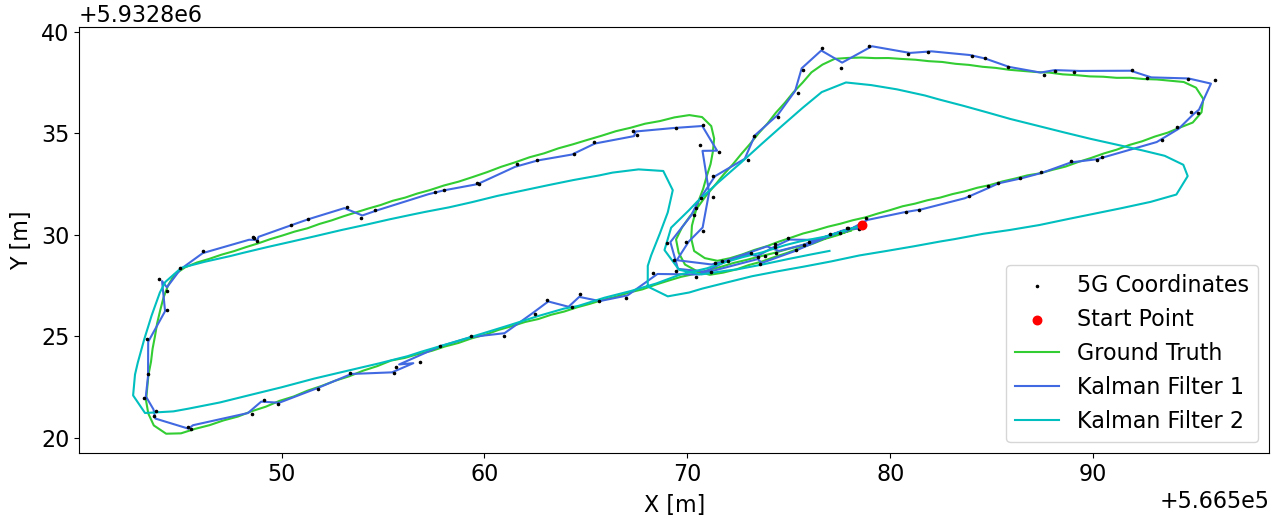
\includegraphics[width=0.8\linewidth]{source/images/kf_11_schlecht}
	\caption{Kalman Filter, 5G Koordinaten ('nfg11') und Ground Truth}
	\label{fig:kf_11_schlecht}
\end{figure} 
Beides sind Beispiele f�r einen schlecht eingestellten Kalman Filter. Die Genauigkeitswerte sollten so eingestellt werden, dass ein guter Kompromiss zwischen PDR und 5G Koordinaten gefunden wird und beide sich gut ausgleichen. In Abbildung \ref{fig:kf_11} ist ein Beispiel mit einigerma�en gut austarierten Genauigkeitswerten. Das Ergebnis ist eine Trajektorie, welche nicht zu sehr auf die teils ungenauen 5G Koordinaten reagiert aber auch nicht auf Dauer von der Ground Truth wegdriftet. 
\begin{figure}[h!]
	\centering
	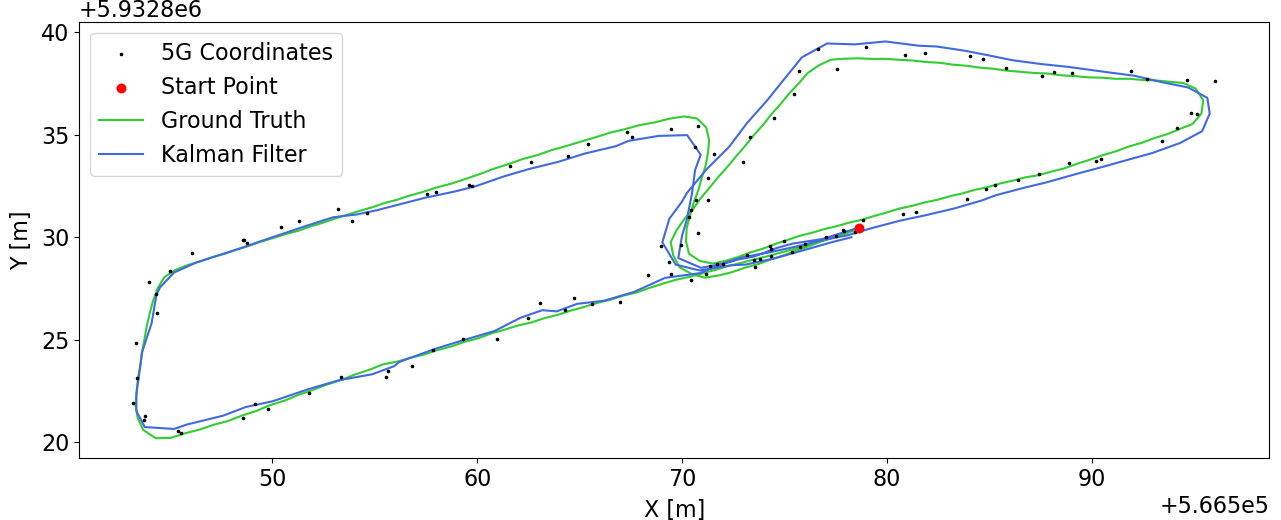
\includegraphics[width=0.8\linewidth]{source/images/kf_11}
	\caption{Kalman Filter, 5G Koordinaten ('nfg11') und Ground Truth}
	\label{fig:kf_11}
\end{figure}
Abbildung \ref{fig:kf_53} zeigt den gleichen Filter allerdings mit dem 5G Datensatz welcher wesentlich weniger Beobachtungen beinhaltet und ungenauer ist. 
\begin{figure}[h!]
	\centering
	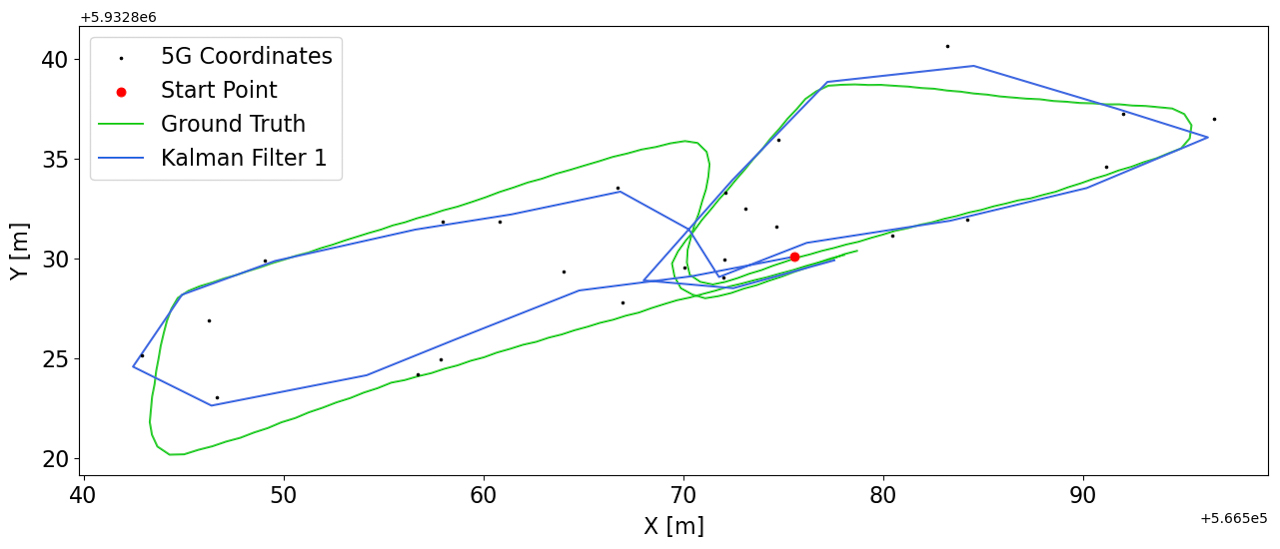
\includegraphics[width=0.8\linewidth]{source/images/kf_53}
	\caption{Kalman Filter, 5G Koordinaten ('nfg53') und Ground Truth}
	\label{fig:kf_53}
\end{figure}
Abbildung \ref{fig:kf_53} zeigt die Trajektorie, welche sich durch den diskreten Kalman Filter ergibt, sowie die 5G Koordinaten und die Ground Truth. Hier ist deutlich zu sehen, dass der Filter nur so viele Punkte hat wie 5G Punkte in den Filter einflie�en. Dadurch wirkt die Trajektorie sehr eckig und wei�t deutlich gr��ere Abweichungen zur Ground Truth auf.
\subsection{Extended Kalman-Filter}
\subsubsection{Ergebnisse}
\subsection{Weighted-Least-Square}
F�r die Implentation der Weighted-Least-Square Methode werden in einem ersten Schritt die 5G Beobachtungen anhand der PDR Beobachtungen interpoliert ($x_i, y_i$), indem aus der Schrittl�nge $L$ und der Schrittrichtung $R$, $\Delta x$ und $\Delta y$ berechnet werden und diese auf die 5G Koordinaten aufaddiert werden.
Je nachdem wie h�ufig eine neue 5G Beobachtung vorliegt wird entweder eine 5G Beobachtung f�r $x_i, y_i$) herangezogen oder der vorangegangene interpolierte 5G Wert. F�r die Schrittrichtung ist die Nordrichtung $\Phi_0$ essentiell, welche f�r den Beispiel Datensatz bei 3.5 rad liegt.
\begin{equation}
x_{i+1} = x_i + L_i \cdot \cos(\Phi_0 + R_i)
\end{equation}
\begin{equation}
y_{i+1} = y_i + L_i \cdot \sin(\Phi_0 + R_i)
\end{equation}
Dieses Interpolieren wird so h�ufig durchgef�hrt, bis eine neue 5G Beobachtung vorliegt. Als Ergebnis liegt nun f�r jede PDR Beobachtung eine 5G Beobachtung bzw. eine interpolierte 5G Beobachtung vor. Dies ist die Voraussetzung f�r das Anwenden der Least-Square-Methode. Anschlie�end k�nnen die Daten in die Sch�tzung der unbekannten Parameter eingehen (siehe Formel \ref{LS}). In der Gewichtsmatrix $P$ findet die Gewichtung der Beobachtungen statt, wobei absolute (5G Koordinaten) und relative Beobachtungen (PDR Werte) unterschiedliche Standardabweichungen und somit Gewichte erhalten. So wird gesteuert, welche Beobachtungen mehr Einfluss bei dem Ausgleich haben sollen und bei welchen die quadratische Verbesserung h�her sein darf. Die Ausgleichung findet bei jedem dazukommenden 5G Punkt neu statt. 

\subsubsection{Ergebnisse}
Dir f�r die Weighted-Least-Square Methode verwendeten Genauigkeiten bilden auf der einen Seite die von den 5G Koordinaten (absolute) und auf der anderen Seite die f�r die PDR Werte (relativen). Das Ergebnis in Abbildung \ref{fig:ls_11} zeigt den Datensatz 'nfg11', der weit aus mehr Beobachtungen hat als der 'nfg53' Datensatz. Hier wurden den PDR Beobachtungen mehr Gewicht gegeben womit sie eine sehr gute Genauigkeit aufweisen ($\sigma_{PDR}$ = 0.2). Im Gegensatz dazu wird den 5G Koordinaten weniger Einfluss in die Ausgleichung gegeben. Ihre Standardabweichung liegt deutlicher h�her als die von den PDR Beobachtungen ($\sigma_{5G}$ = 3).  
\begin{figure}[h!]
	\centering
	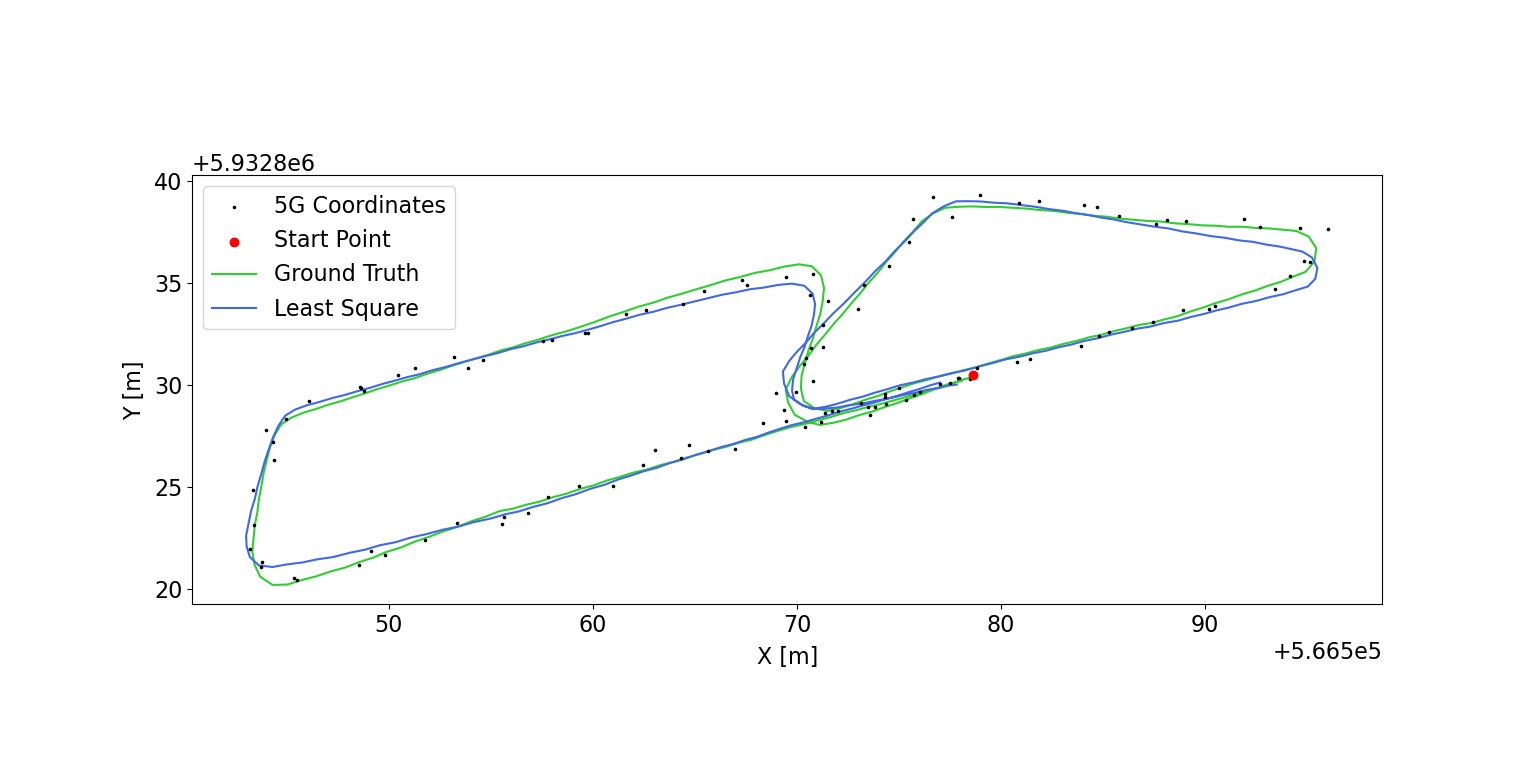
\includegraphics[width=0.8\linewidth]{source/images/ls_11}
	\caption{WLS, 5G Koordinaten ('nfg11') und Ground Truth}
	\label{fig:ls_11}
\end{figure}
\begin{figure}[h!]
	\centering
	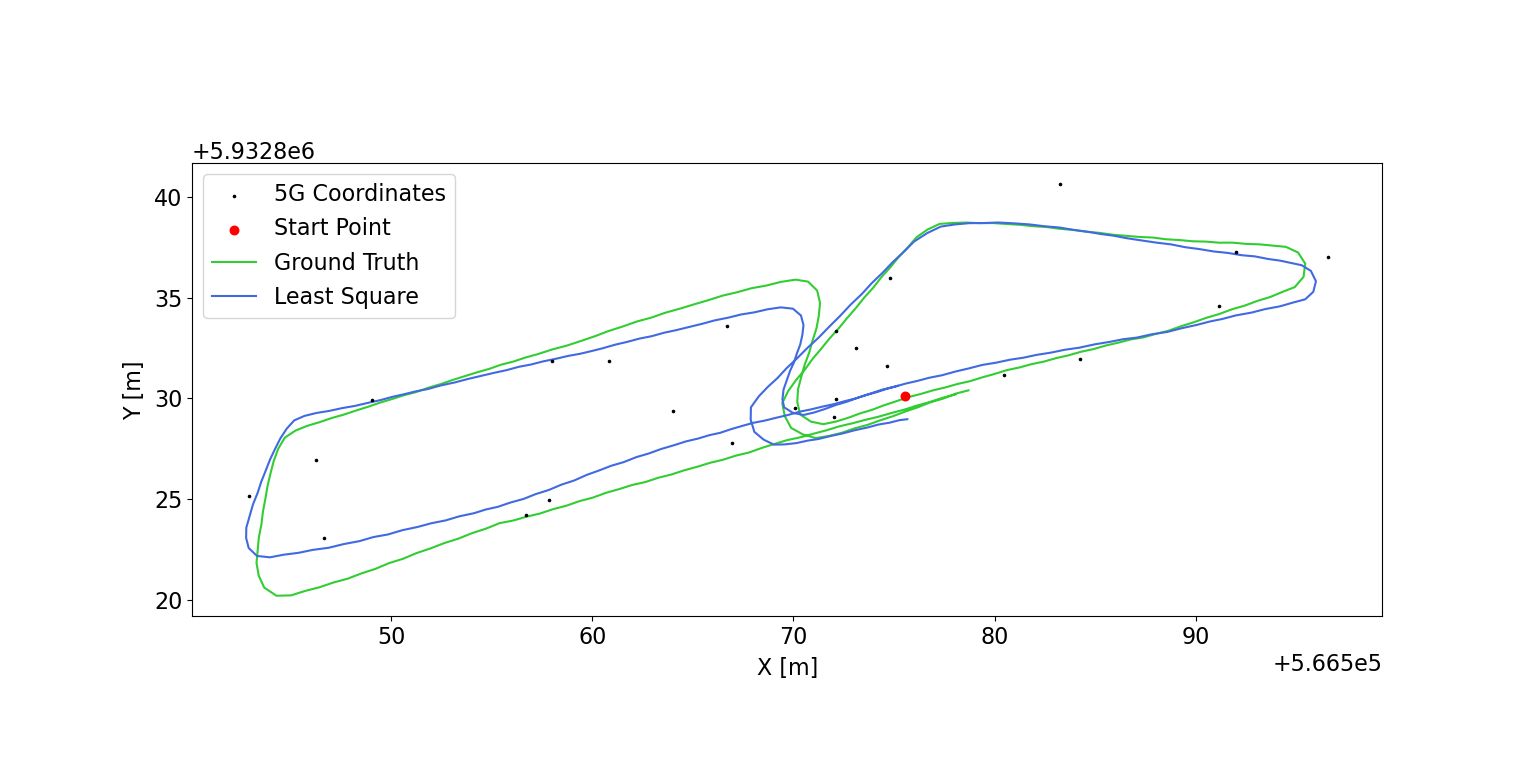
\includegraphics[width=0.8\linewidth]{source/images/ls_53}
	\caption{WLS, 5G Koordinaten ('nfg53') und Ground Truth}
	\label{fig:ls_53}
\end{figure}
Das Ergebnis zeigt, dass der Verlauf der WLS Ausgleichung der eigentlichen Wahrheit entspricht. Nur an einigen Kurvenbereichen gibt es einen kleinen Versatz. Das gleiche Muster ist auch in der Abbildung \ref{fig:ls_53} zu sehen. Obwohl dieser Datensatz eine geringe Menge an Beobachtungen aufweist als der zuvor, kann hier auch beobachtet werden, dass der grobe Verlauf der tats�chlichen Trajektorie entspricht. Die Einstellung der Standardabweichung sowohl f�r die 5G Koordinaten als auch f�r die PDR Beobachungen sind unver�nderlich. Sie entsprechen also den gleichen wie bereits in Abbildung \ref{fig:ls_11} zu sehen ist. 

\subsection{Vergleich der Ergebnisse}
Abbildung \ref{fig:vergleich_2} und \ref{fig:vergleich_3} zeigen den Vergleich von Weigthed-Least-Square und dem Kalman Filter mit der Ground Truth bei beiden 5G Datens�tzen. Beim 'nfg11' Datensatz zeigen sich beide Trajektorien relativ gut, lediglich beim rechten Teil zeigt der Kalman Filter etwas gr��ere Differenzen zur Ground Turth als WLS. Beim schlechteren 'nfg53' Datensatz werden die Unterschiede schon etwas gr��er.
\begin{figure}[h!]
	\centering
	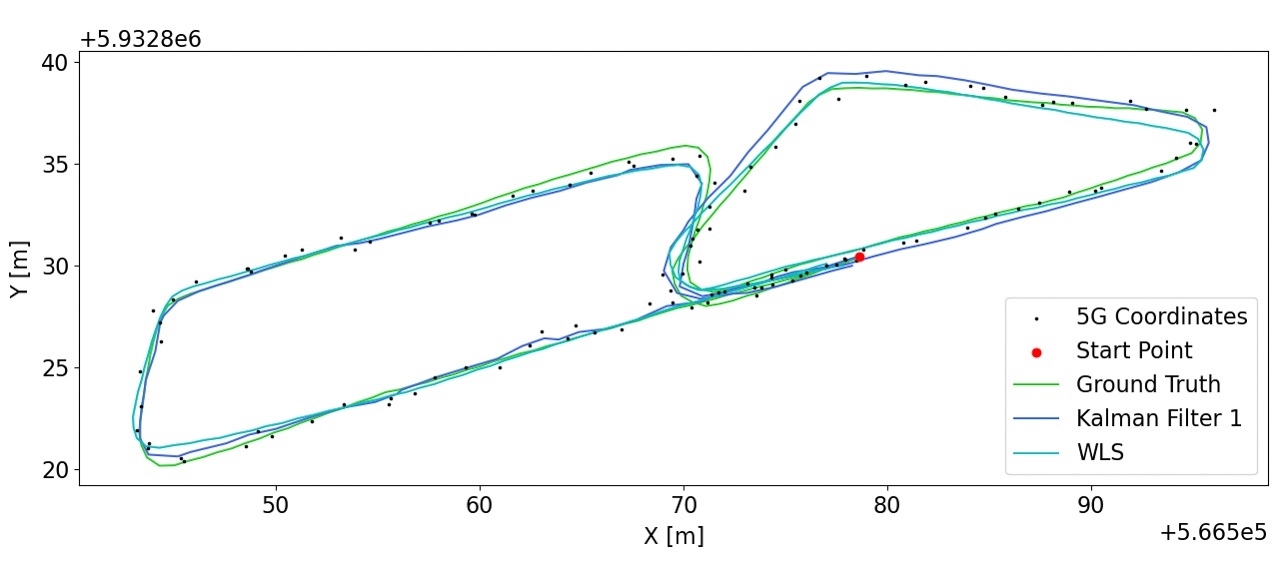
\includegraphics[width=0.8\linewidth]{source/images/vergleich_ls_kf_11}
	\caption{Vergleich zwischen Kalman Filter und WLS ('nfg11')}
	\label{fig:vergleich_2}
\end{figure}
\begin{figure}[h!]
	\centering
	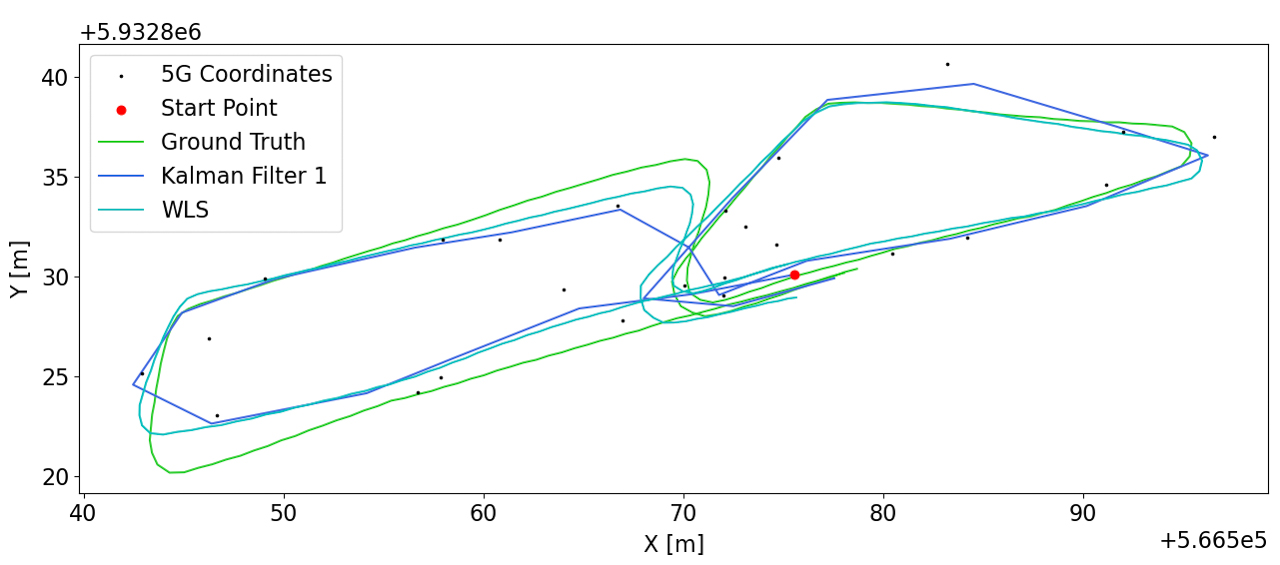
\includegraphics[width=0.8\linewidth]{source/images/vergleich_ls_kf_53}
	\caption{Vergleich zwischen Kalman Filter und WLS ('nfg53')}
	\label{fig:vergleich_3}
\end{figure}

Vergleicht man den Kalman Filter mit der Weighted-Least-Square Methode so f�llt auf, dass der Kalman Filter insgesamt viel eckiger ausf�llt als die vergleichsweise runde Trajektorie von WLS. Gerade beim 'nfg53' Datensatz wird dies deutlich. Dies liegt daran, dass der Kalman Filter nur bei jeder neuen 5G Beobachtung updatet und eine neue Position berechnet. Abbildung \ref{fig:vergleich_1} verdeutlicht dies. Hier wurde eine gr��ere Beobachtungsl�cke simuliert bei der die Ground Truth zwei Kurven zur�cklegt. W�hrend der Kalman Filter fast auf direktem Weg zur n�chsten 5G Beobachtung abk�rzt, simuliert die Least-Square Trajektorie die beiden Kurven einigerma�en gut. Hier schneidet die WLS Methode besser ab als der Kalman Filter.
\begin{figure}[h!]
	\centering
	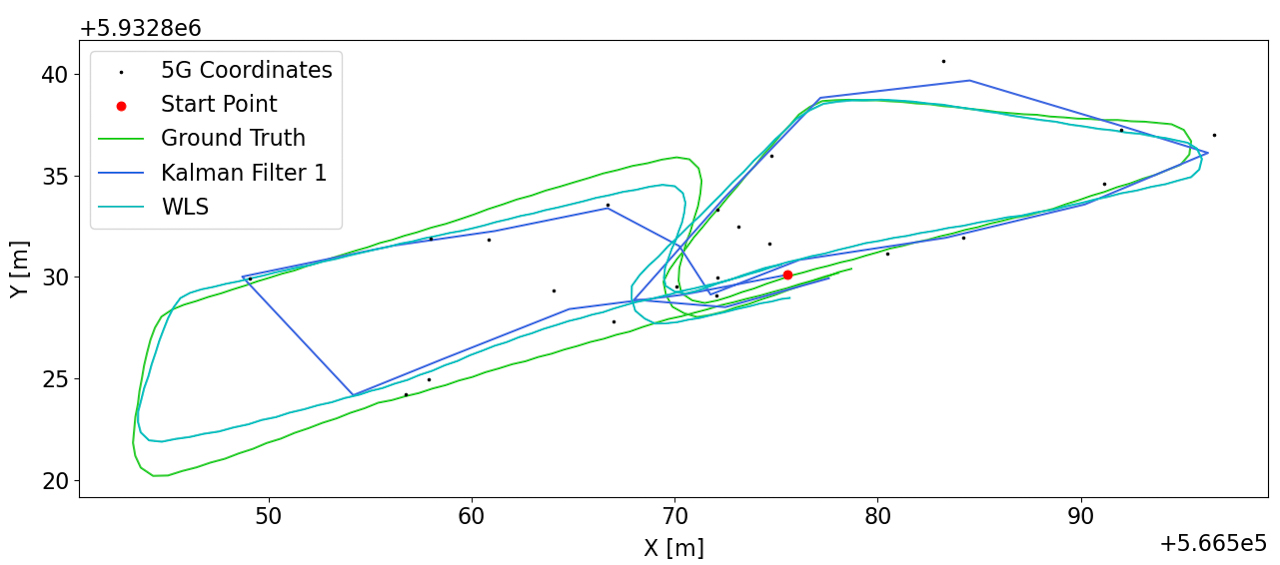
\includegraphics[width=0.8\linewidth]{source/images/vergleich_ls_kf_gap}
	\caption{Vergleich zwischen Kalman Filter und WLS bei Beobachtungsl�cke}
	\label{fig:vergleich_1}
\end{figure}

\section{Fazit und Ausblick}
\textcolor{red}{Eine Er�rterung (oder "Bewertung") der Ergebnisse, Zusammenfassung und zuk�nftige Forschungsperspektiven}

Zusammenfassend kann vorab festgehalten werden, dass die Trajektorie der Weighted-Least-Square Methode besser abschneidet als die des diskreten Kalman Filters. Das zeigt sich auch noch mal an der Abbildung \ref{fig:vergleich_1}, in der eine Beobachtungsl�cke simuliert wurde. Dadruch das die WLS Methode interpolierte 5G Werte mit in die Ausgleichung nimmt, kann die gesamte Trajektorie besser bestimmt werden als bei dem diskreten Kalman Filter. 

Als zuk�nftige Forschungsperspektive k�nnte der Extended Kalman Filter noch mehr erweitert werden. Der Vektor der gesch�tzten Parameter $\boldsymbol{\hat{x}}_{i}$, der eine Dimension von 4x1 aufweist k�nnte auf eine Dimension von 6x1 erweitert werden. Daf�r kommen neben dem ${x}_{i}$, ${y}_{i}$, ${L}_{i}$ und ${R}_{i}$ noch die Fehler der Schrittl�nge und -richtung ($L_{error_i}$,$R_{error_i}$) hinzu. Es wird vermutet, dass durch Ber�cksichtigungen der Ungenauigkeit f�r Schrittl�nge und -richtung das Vorhersage noch besser funktionieren. Ob das der Wirklichkeit entspricht, kann dieser Ansatz in Zukunft �berpr�ft werden. 

%\bibliography
\addcontentsline{toc}{section}{Literatur}
%\printbibliography[title = Literaturverzeichnis]

\bibliographystyle{IEEEtran}
\bibliography{sampleBibFile}
\end{document}


